\documentclass[aps,pre,twocolumn,showpacs,amsmath,amssymb]{revtex4-1}

\usepackage{graphicx}
\usepackage{color}

\usepackage[portuguese]{babel}
\usepackage[utf8]{inputenc}
\usepackage[T1]{fontenc}

\usepackage{titlesec}

\setlength{\belowcaptionskip}{-2pt}

\titlespacing*{\section}{0pt}{\baselineskip}{\baselineskip}
\titlespacing*{\subsection}{0pt}{\baselineskip}{\baselineskip}

\hfuzz 1pt
\vfuzz 1pt

\setlength{\parskip}{\baselineskip}

\begin{document}

\title{Exercício 2: Raízes de funções}

\author{Rita Soares, Ernesto González, Raquel Cabrera}

\begin{abstract}
  Cálculo de raízes de funções pelos métodos da bisseção, de Newton e da secante. Cálculo de $\sqrt{4}$ e estudo da sucessão de erros absolutos para os diferentes métodos. Cálculo de $9e^{-t}sin(2\pi t)=1.5$ usando o método de Newton. Estudo das raízes de $y=tan(\theta_0)x-\frac{g}{2v_{0}^{2}cos^2(\theta_0)}x^2+y_0$.
\end{abstract}

\maketitle

\section{Raiz quadrada de um número}

Para calcular $\sqrt{4}$ defina-se a função $f(x)=x^2-4$, cujas raízes são as
raízes quadradas de $4$. \\
Aplique-se o método da bissecção para encontrar as raízes de $f$, partindo dos
intervalos $[0.7,2.6]$, $[0.4,1.7]$ e $[-3,0.6]$ e usando como critério de
convergência $\epsilon = 10^{-5}$. Os resultados obtidos são apresentados na
Figura 1.

\begin{figure}[h]\vspace{-2ex}
   \begin{center}
    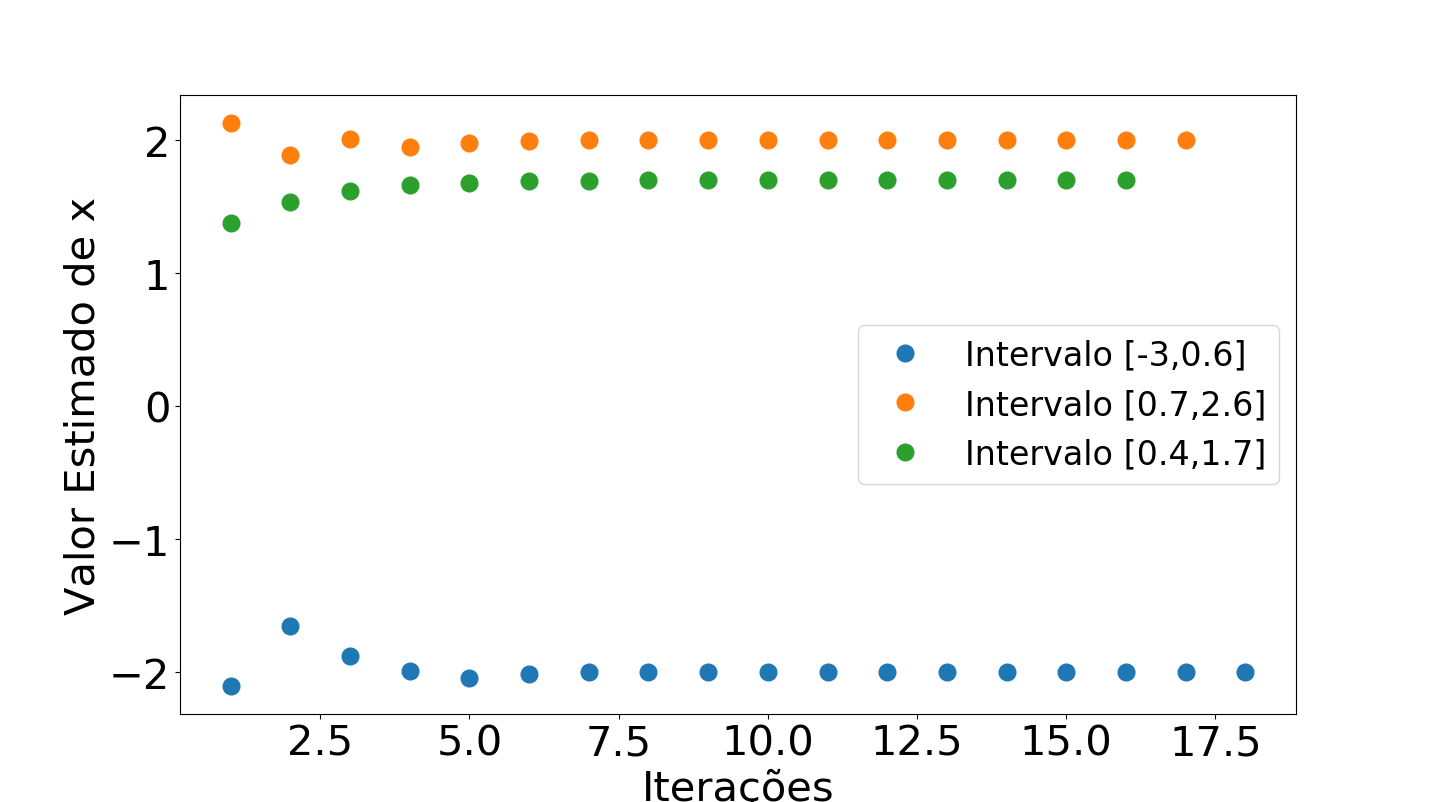
\includegraphics[width=\columnwidth]{Figure_1.png} \\
\caption{Gráfico do valor estimado da raiz em função do número de iterações, usando o método da bissecção na função $x^2-4$ (gerado em Python).}
  \label{fig.exemplo}
   \end{center}
\end{figure}

Na Figura 1 estão representadas as aproximações às raízes de $f$ em função do número de iterações. Nos intervalos $[0.7, 2.6]$ e $[-3, 0.6]$ as curvas tendem para $x=2$, com 17 iterações, e $x=-2$, com 18 iterações, respetivamente. Correspondem, assim, às raízes de $f$. Contudo, no intervalo [0.4, 1.7], a curva converge para aproximadamente $x=1.7$, após 16 iterações. Isto deve-se à natureza do método da bisseção: os pontos iniciais $a$ e $b$ devem ser tais que $f(a)<0$ e $f(b)>0$ para garantir a existência de uma raiz de $f$ em $[a,b]$. Veja-se que $f(0.4)<0$
e $f(1.7)<0$, não cumprindo as condições iniciais do método. No caso em que não há raízes no intervalo inicial, as aproximações às raízes convergem, geralmente, ao extremo do intervalo que tem imagem mais perto de $0$. No caso de $[0.4,1.7]$, temos $|f(1.7)|<|f(0.4)|$, daí as aproximações à raiz convergirem para $1.7$.\\
As aproximações encontradas na segunda iteração, tanto para o intervalo $[0.7,2.6]$ como para $[-3,0.6]$, estão desalinhadas em relação aos valores vizinhos. Deve-se às grandes amplitudes dos intervalos iniciais, que, aliadas ao declive pronunciado da função quadrática longe do vértice da parábola, vão fazer com que a diferença entre as aproximações às raízes nas iterações 1 e 2 estejam muito afastadas. \\
As oscilações das aproximações à volta das raízes para $[-3,0.6]$ e $[0.4,1.7]$ deve-se à gradual aproximação às verdadeiras raízes à medida que o método descarta os valores mais distantes a $Ox$ e encontra novos valores de um lado e do outro do eixo $Ox$ ao calcular o ponto médio dos atuais.\\

Acima foi usado o método da bisseção para calcular aproximações às raízes de $f$. Usando o método de Newton obtemos $x=2.00000000027836$ e pelo método da secante $x=1.9999999913282793$.
Uma das desvantagens do método da bisseção é a sua lenta convergência às raízes. Na Figura 2 relaciona-se o logaritmo do erro absoluto em função do número de iterações para o método da bisseção, o método de Newton e o método da secante.

\begin{figure}[h]\vspace{-7ex}
   \begin{center}
    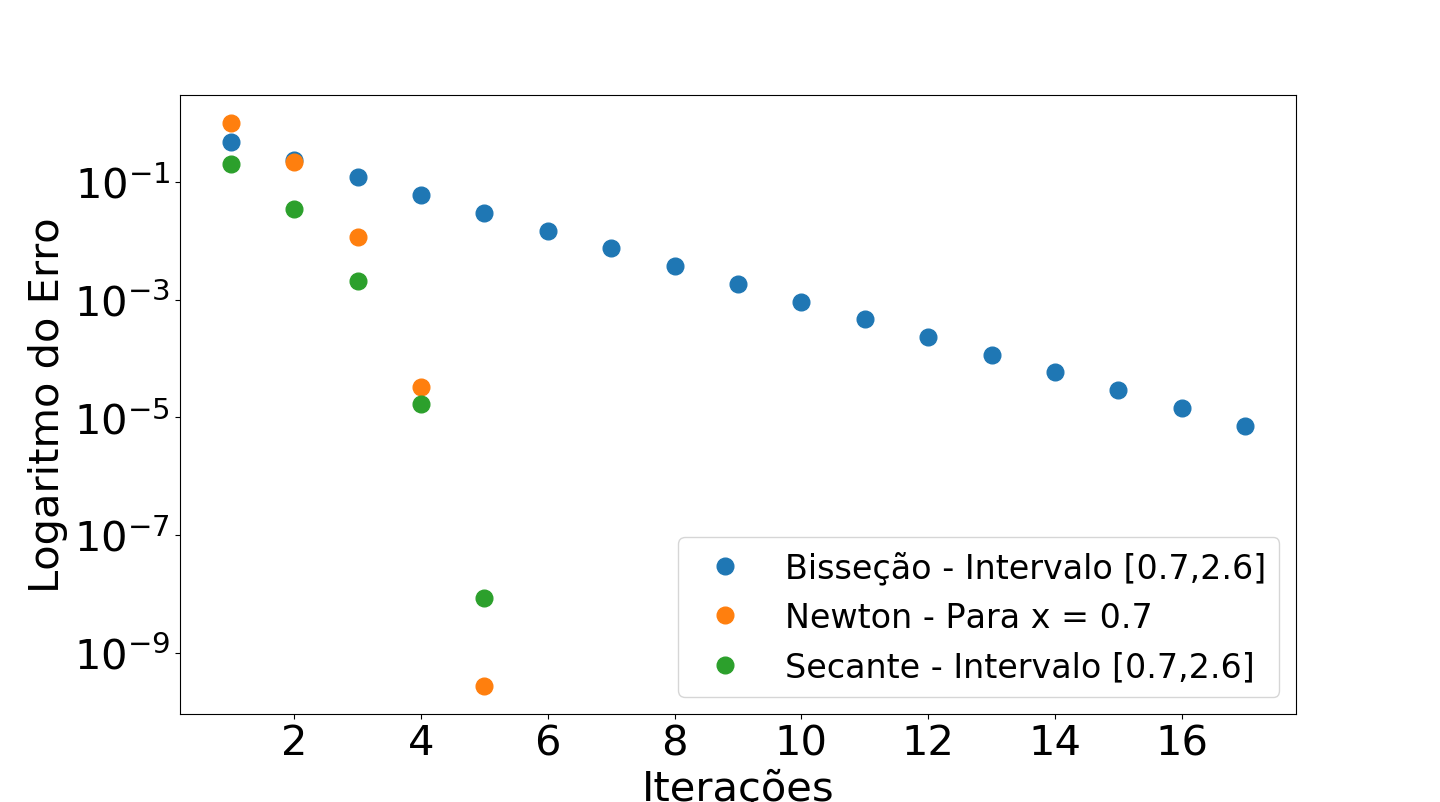
\includegraphics[width=\columnwidth]{Figure_2.png} \\
\caption{Gráfico do logaritmo do valor absoluto do erro do método indicado em função do número de iterações (gerado em Python).}
  \label{fig.exemplo}
   \end{center}
\end{figure}

Pode-se observar um menor erro absoluto final no método de Newton. Neste caso, o método de Newton e o método da Secante atingem o critério de convergência ($\epsilon=10^{-5}$) ao cabo de apenas 5 iterações. O método da bisseção leva 17 iterações e o seu erro absoluto final é maior que o dos outros dois métodos.



\section{Corrente oscilante em circuitos}

Considere-se a corrente de um circuito definida pela função
\begin{equation}
    I(t)=9e^{-t}sin(2\pi t)-1.5
\end{equation}
Na Tabela I encontram-se as raízes encontradas usando o método de Newton de acordo com o valor inicial estabelecido. Os valores $x_{Python}$ foram calculados usando método de Newton simples, os valores $x_{Mathematica}$ usando o método de Newton com \textit{Step Control} - algoritmo de controlo do salto que impede a repetição ou a saída de zonas próximas de raízes ou mínimos.
\begin{table} [h]
  $$\begin{array}{|c|c|c|c|} \hline
  t_0 & \text{Iterações} & t_{Python} & t_{Mathematica} \\ \hline
  0.6 & 3 & 0.4575814699215208 & 0.457582 \\ \hline
  0.7 & 4 & -0.5158617879572158 & 1.08181 \\ \hline
  0.75 & 11 & -6886.361154309897 & 1.38416 \\ \hline
  0.8 & 6 & 1.3841631272932045 & 1.38416  \\ \hline
  0.9 & 3 & 1.08180661316330885 &  1.08181 \\ \hline
\end{array}$$
  \caption{Raízes encontradas usando o método de Newton de acordo com o valor inicial. A coluna $t_{Python}$ apresenta valores encontrados com algoritmos implementados em Python e a coluna $t_{Mathematica}$ apresenta valores encontrados com a função \textit{FindRoot} do \textit{Mathematica}.}
\end{table}
Vemos como as raízes encontradas para $t_0=0.7$ e $t_0=0.75$ usando Python e \textit{Mathematica} diferem significativamente. Isto deve-se ao método implementado. A raiz estimada em cada iteração é da forma
\begin{equation}
    t_k = I(t_{k-1}) - \frac{I(t_{k-1})}{I'(t_{k-1})}.
\end{equation}
e $I(t_0)=9e^{-t_0}sin(2\pi t_0)-1.5$. A derivada na vizinhança de $t_0=0.75$ é quase nula, o que faz com que
inicialmente os valores encontrados pelo método se afastem da zona com raiz em que estavam inicialmente. Nas iterações seguintes, estes valores vão saltando entre zona e zona até que, na 10ª iteração divergem para $t_{10}=12.41953670040136$. Na iteração seguinte, o valor encontrado afasta-se ainda mais das zonas de raízes: $t_{11}=-6886.361154309897$. Ao calcular a raiz estimada para a próxima iteração, $I(t_{11})$ e $I'(t_{11})$ envolvem esponenciais de $-t_{11}$. Veja-se como $e^{6886.361154309897}>e^{1024}$, com $e^{1024}$ o maior exponencial representável na máquina de Python, justificando-se o erro de Overflow na iteração seguinte e forçando a paragem do método.\\
Para $t_0=0.7$, também na 1ª iteração os valores encontrados saem da zona de raízes em que se encontravam inicialmente e, já na 2ª iteração converge para $t_2= -0.5126791910862967$, que se encontra na vizinhança de uma raiz de $I(t)$. Até à 4ª iteração o método vai convergir para $t_4=-0.5158617879572158$, nunca tendo saído da zona de raiz encontrada na segunda iteração.



\section{Projétil sem atrito}
Considere-se um projétil cuja trajetória é descrita por
\begin{equation}
  y=tan(\theta_{0})x-\frac{g}{2v_{0}^{2}cos^2(\theta_{0})}x^2 + y_0
\end{equation}
para $y_0=1\,m$, $v_0=30\,ms^{-1}$.\\
\subsection{Atingir um alvo em $y=1.8\,m$ e $x=90\,m$}
Considere-se, agora, que se pretende atingir um alvo que se encontra em $y=1.8\,m$ e $x=90\,m$. Substituindo em (3), e sabendo que $g=9.81$, vem
\begin{equation}
  0=90\,tan(\theta_0)- \frac{44.145}{cos^2(\theta_0)}-0.8.
\end{equation}
Para resolver a equação utilizou-se o método da secante. Observe-se os resultados na Tabela II.
\begin{table} [h]
  $$\begin{array}{|c|c|c|c|c|} \hline
  \theta_0 & \theta_0^0 & \theta_0^1 & \text{Iterações} & \text{Precisão} \\ \hline
  0.7185431686476985 & 0.8 & 0.7 & 4 & 10^{-6} \\ \hline
  0.8611426749381886 & 0.8 & 0.85 & 5 & 10^{-6} \\ \hline
  0.7185417844417982 & 0.7 & 0.6 & 4 & 10^{-6} \\ \hline
  3.8601349108796055 & 2 & 2.3 & 10 & 10^{-6} \\ \hline
  4.002735330289595 & 4 & 5 & 5 & 10^{-6} \\ \hline
\end{array}$$
  \caption{Valores $\theta_0$ encontrados usando o método da secante para diferentes valores iniciais escolhidos, com respetivos número de iterações até chegar ao valor e precisão do resultado.}
\end{table}
\subsection{Altura como função de $\theta_0$ e $x$}
Consideremos agora o caso em que $y=y(\theta_0,x)$.
De (3) vem
\begin{equation}
  y(\theta_0,x)=tan(\theta_{0})x-\frac{g}{2v_{0}^{2}cos^2(\theta_{0})}x^2 + 1.
\end{equation}
Procuramos soluções de $y(\theta_0,x)=1.8$.
Encontram-se representados na Figura 3 os resultados.
\begin{figure} [h]
  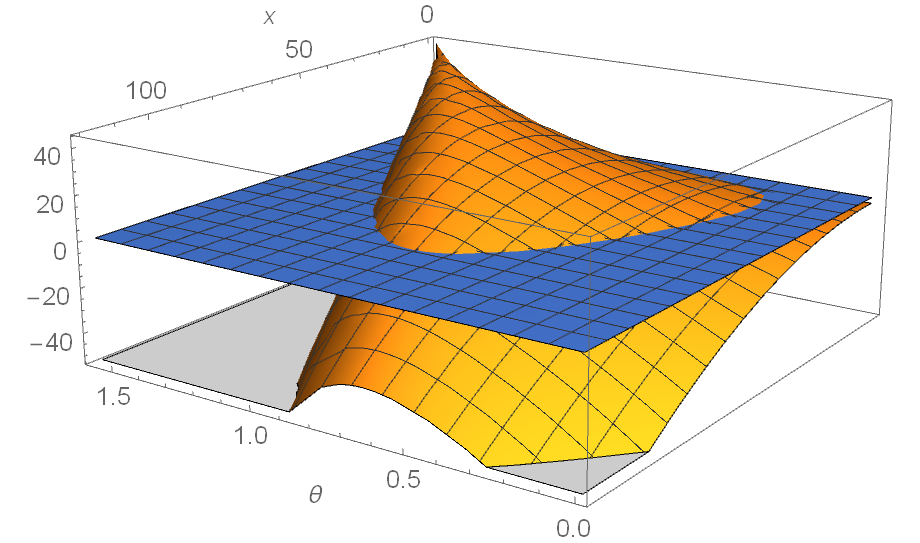
\includegraphics[scale=0.28]{parte3Alineab.png}
  \caption{Representação gráfica de $y=y(\theta_0,x),\;\theta \in [0,\pi/2[,\;x \in [0,120]$ e do plano $y=1.8$. A interseção dos dois é um conjunto de pares $(\theta_0,x)$ solução de (1) para $y=1.8$}
  \label{}
\end{figure}
\end{document}
